%% ----------------------------------------------------------------------------
% CVG SA/MA thesis template
%
% Created 03/08/2024 by Tobias Fischer
%% ----------------------------------------------------------------------------

% General instructions:
% Give an introduction to the topic you have worked on:

% \begin{itemize}
 % \item \textit{What is the rationale for your work?} Motivate the problem, \eg with a general description of the problem setting, narrowing down to the particular problem you have been working on in your thesis. Allow the reader to understand the problem setting. 
 % \item \textit{What is the technical gap in existing work?} Briefly outline how this problem has been tackled before, and what the shortcomings of the existing solutions are.
 % \item \textit{What is your work doing to fix it?} Given the above background, state briefly the focus of the work. 
% \end{itemize}


\chapter{Introduction}
In his essay on \emph{The Bitter Lesson}, Richard Sutton argues that, in the long run, scaling computation and data tends to outperform solutions that are heavily hand-engineered for a specific domain \cite{bitterlesson}. In computer vision, this shift is visible in the growing role of pretrained models as general priors: many pipelines now rely on large models that already encode strong assumptions about images, motion, and geometry. At the same time, these pipelines still make use of significant domain knowledge in their design and often rely on per-scene optimization to achieve high-quality results, especially in ill-posed settings such as monocular 4D reconstruction.

In parallel, there is a growing line of feed-forward reconstruction models that map monocular video directly to a 3D/4D representation without per-scene optimization, which is closer in spirit to Sutton's lesson. These models promise high throughput, which is appealing for applications such as robotics. Figure~\ref{fig:ours_vs_feedforward} illustrates that they still lag behind optimization-based methods in reconstruction quality, especially in challenging dynamic scenes.

A key bottleneck for feed-forward 4D reconstruction methods is training data, which remains scarce for real-world dynamic scenes. This motivates hybrid methods that exploit pretrained priors while still performing targeted per-scene refinement at a practical runtime. In this thesis, we explore one such hybrid pipeline for human-centric 4D reconstruction from monocular video. We initialize the scene from off-the-shelf estimates and then refine pose and appearance with a lightweight optimization stage. We hope that, beyond enabling new applications, this pipeline can also act as a step towards producing higher-quality dynamic 4D supervision for training stronger feed-forward models in the future.

\begin{figure}[!ht]
    \centering
    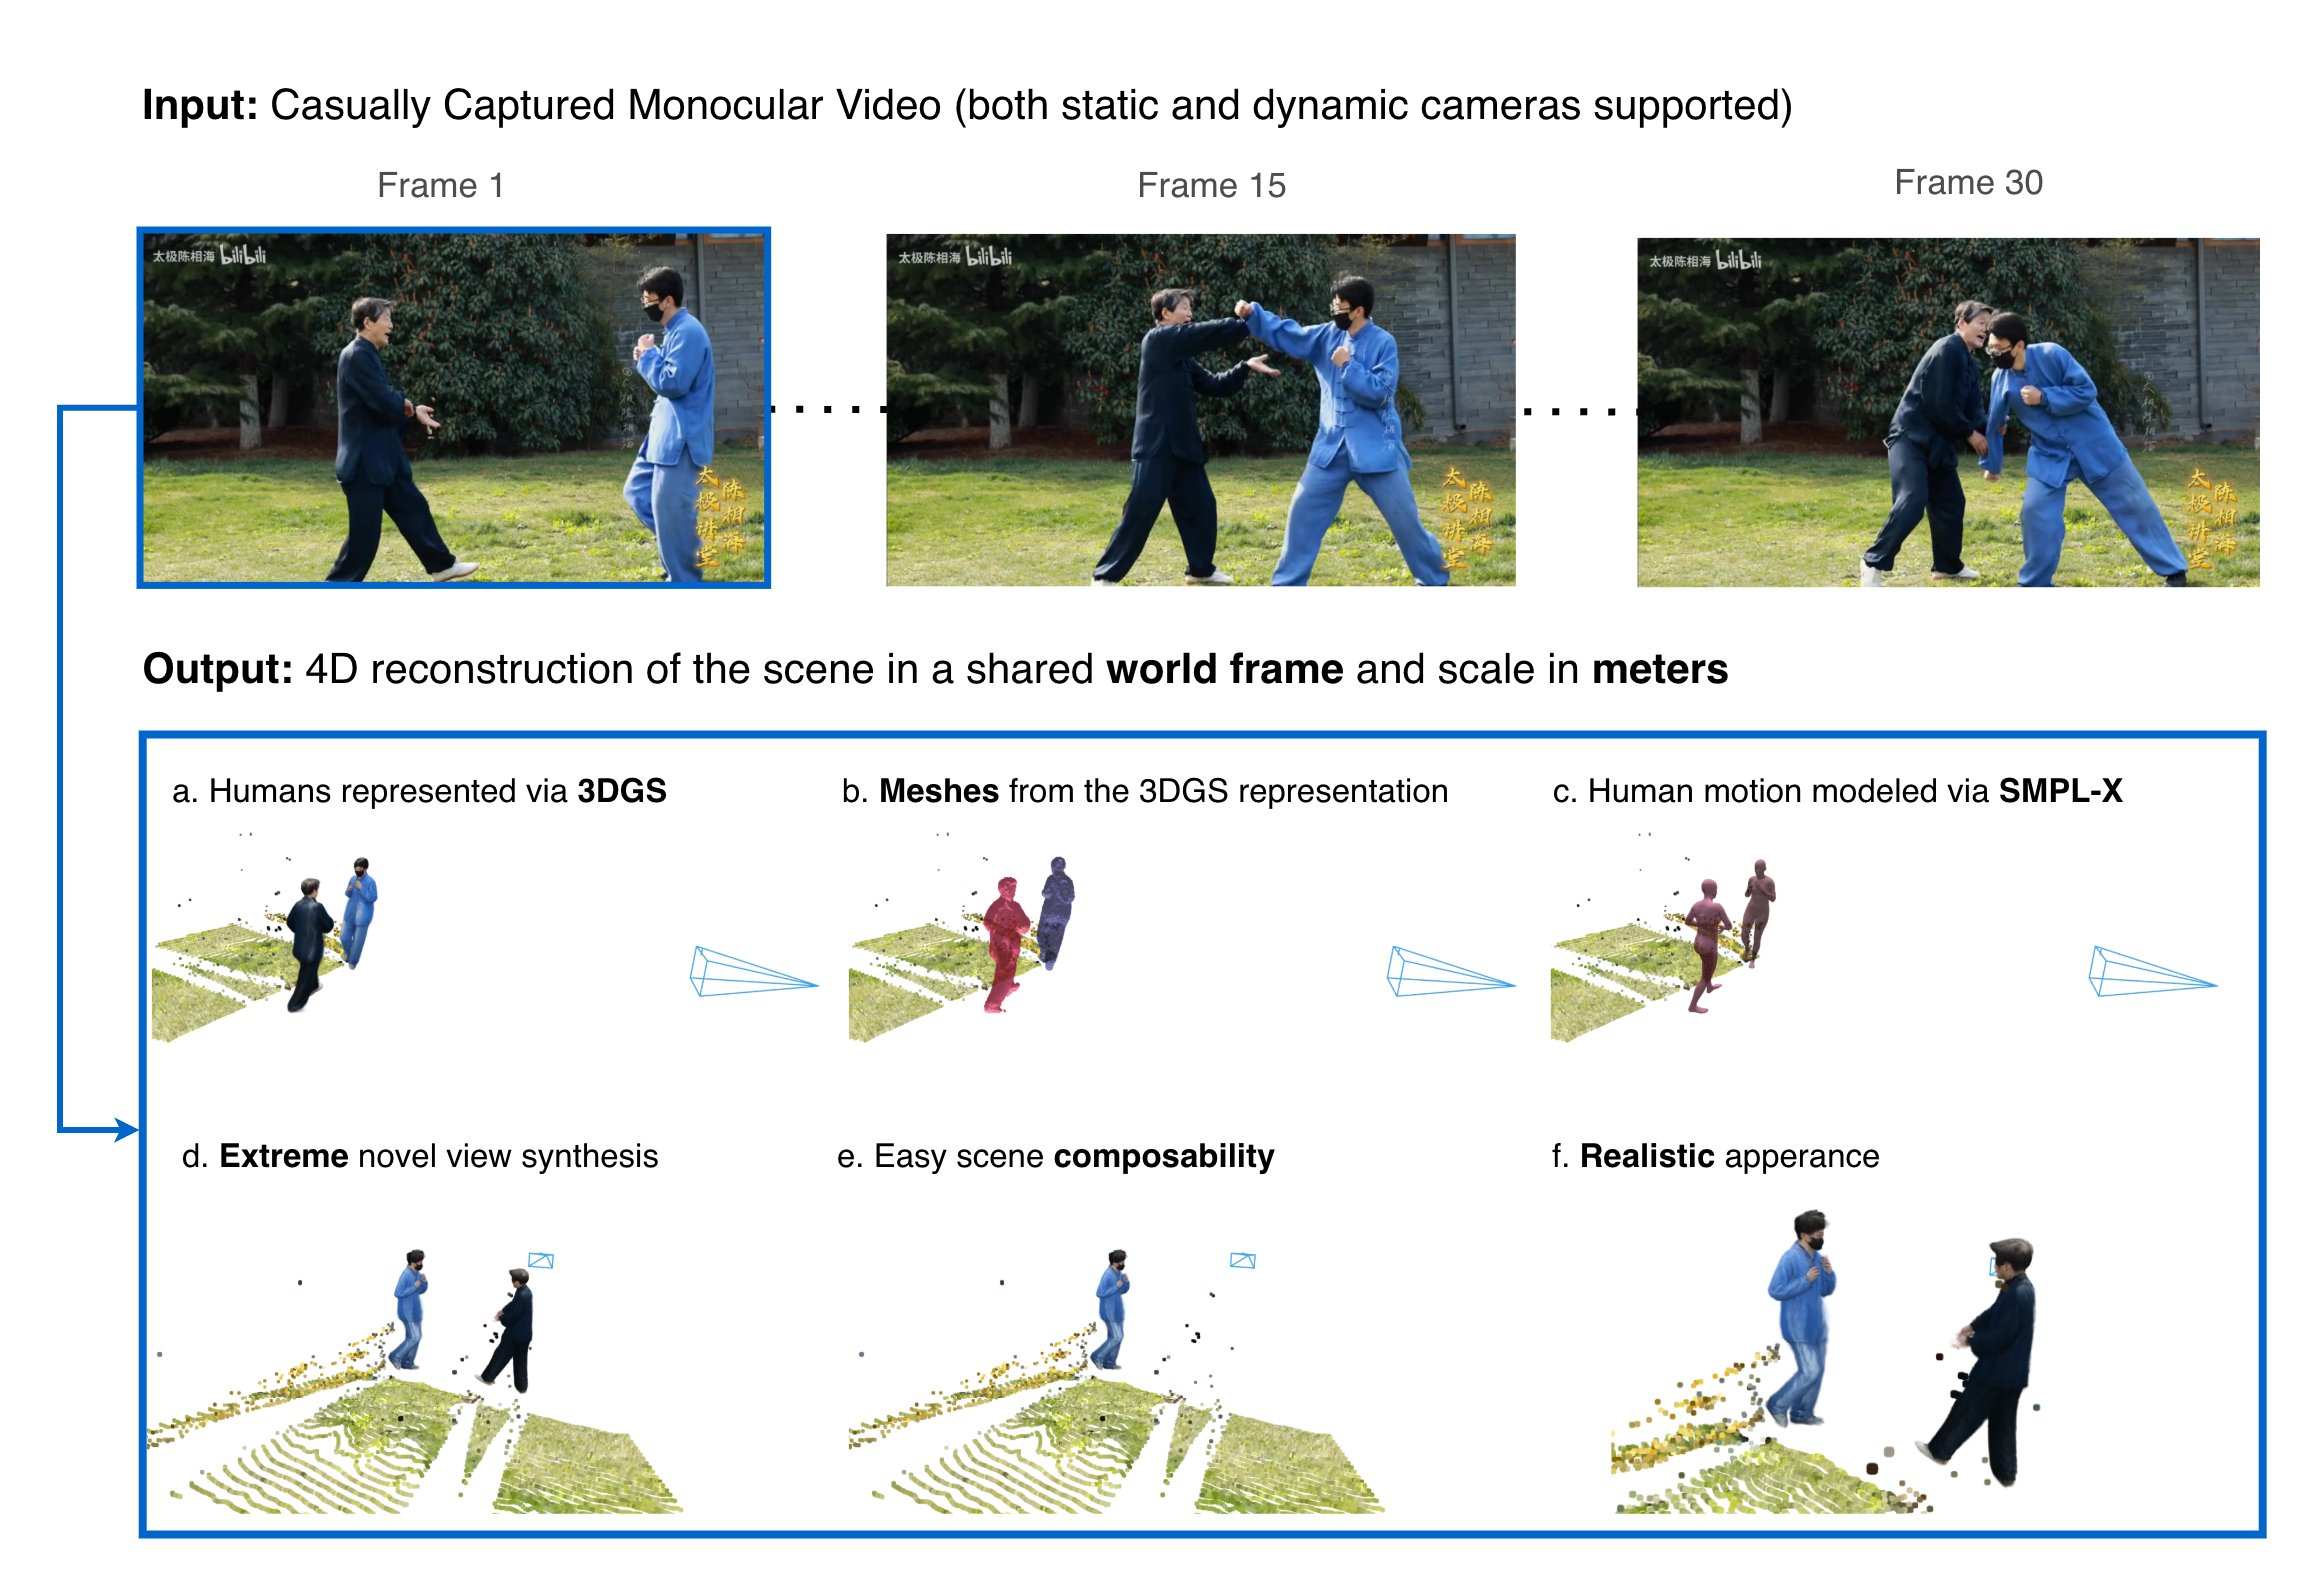
\includegraphics[width=1.0\textwidth]{figures/what_our_method_does_impress_fig.drawio.png}
    \caption{\textbf{High-level overview of our method}. We propose a hybrid framework for monocular 4D reconstruction of dynamic human-centric scenes that combines feed-forward priors with targeted per-scene optimization. Given a monocular video, our method produces a renderable 4D representation that supports novel view synthesis and human motion analysis.}
    \label{fig:input_output_overview}  
\end{figure}


Concretely, we focus on reconstructing dynamic human-centric scenes from monocular video, including both static and moving cameras, and settings with multiple interacting people. As Figure~\ref{fig:input_output_overview} illustrates, our method outputs a consistent 4D representation with metric scale. We represent each person with an explicit 3D Gaussian Splatting (3DGS) model whose motion is driven by the SMPL-X body model \cite{smplx}. This alignment with SMPL-X supports downstream motion analysis, for example markerless motion capture and motion retargeting in humanoid robotics (e.g., VideoMimic \cite{videomimic}). In addition, the explicit representation supports novel view rendering of the dynamic humans, which is relevant for free-viewpoint video and interactive media, including creative production workflows.

In practice, reconstructing a dynamic scene from monocular video is highly ill-posed and requires many coupled subproblems to be solved consistently. The system must disentangle camera motion from object motion, maintain temporal stability, and produce view-consistent geometry and appearance while hallucinating unseen regions. For human-centric scenes, the difficulty increases further: humans are non-rigid, they frequently self-occlude and occlude each other, and plausible reconstructions require valid body shape and pose even under ambiguous observations. 

However, existing human-centric methods often focus on reconstructing a single high-quality avatar only from a cleanly captured single image, a set of images \cite{anigs,gas,qiu2025lhm}, or from monocular video \cite{humannerf,neuman,guo2023vid2avatar,exavatar}. In contrast, we target scenes with multiple people who may interact, occlude each other, and perform complex motions, which introduces additional ambiguity and error modes. There are prior attempts closer to our setting, most notably MultiPly \cite{multiply} and Guess The Unseen \cite{gtu}, but these pipelines rely on heavy per-scene optimization and can require hours to days of compute per scene, making them harder to use in practical workflows.

Besides parametric-model-based pipelines (SMPL \cite{smpl} and SMPL-X \cite{smplx}), there are also more general approaches such as Shape-of-Motion \cite{som}, which use pretrained tracking models to define deformation fields without an explicit human body prior. While these methods are appealing for their generality, the resulting humans can have weaker pose and shape quality than approaches that explicitly constrain motion with a parametric body model, especially under occlusion and close interactions.

\begin{figure}[!ht]
    \centering
    \includegraphics[width=1.0\textwidth]{figures/qual_feedforward_vs_ours.drawio.png}
    \caption{\textbf{Comparison of feed-forward method reconstruction and our hybrid method}. Current state-of-the-art feed-forward V-DPM \cite{vdpm} produces subpar geometry and appearance on challenging dynamic scenes with multiple people compared to our hybrid method, which combines feed-forward priors with per-scene optimization.}
    \label{fig:ours_vs_feedforward}  
\end{figure}

Therefore, given the limitations of existing methods and the current challenges in the 4D reconstruction field, the main contributions of this work are:
\begin{itemize}
    \item A hybrid framework for monocular 4D reconstruction of dynamic human-centric scenes that combines feed-forward human and camera priors with targeted per-scene optimization of an explicit 3DGS representation.
    \item A renderable representation aligned with SMPL-X \cite{smplx}, enabling both novel view synthesis and human motion analysis from monocular video.
    \item An exploration of two practical design choices for multi-person monocular reconstruction: using a more expressive body model (SMPL-X) and using generative refinement for view densification, motivated by limitations of prior optimization-heavy methods such as MultiPly \cite{multiply}.
    \item An experimental evaluation across pose estimation, novel view synthesis, mesh reconstruction, and training speed on Hi4D and MMM, highlighting strengths and remaining limitations of the approach.
\end{itemize}
